\chapter[Verwendung]{Verwendung der FM3D-Engine}
Die Flying-Mind 3D Engine ist eine Spiel-Engine für die Entwicklung von Computerspielen. Die Flying-Mind 3D Engine besteht aus zwei Teilen: aus einer dynamischen C++ Bibliothek und dem Designer, einer grafische Nutzeroberfläche. Der Spieleprogrammierer verwendet die Bibliothek, um die Logik des Spiels zu beschreiben und den Designer, um Entities zu erstellen und Ressourcen des Spiels zu verwalten, wie Modelle und Texturen. Die Nutzung des Designers ist komplett optional. Es ist möglich ein vollständiges Spiel ohne den Designer zu programmieren. Dies wird aber nicht empfohlen. 

\section{Mindestvorraussetzungen...}
\subsubsection{...für den Computer, auf welchem später das Spiel gespielt wird:}
\begin{itemize}
	\item Windows 32-Bit/64-Bit
	\item OpenGL 3.3 oder höher
\end{itemize}
\subsubsection{...für den Computer, auf welchem der Designer ausgeführt wird:}
\begin{itemize}
	\item Windows 32-Bit/64-Bit
	\item OpenGL 3.3 oder höher
	\item .Net 4.5
	\item Visual Studio 15
	\item (Für einen Debug des Spiels müssen die Voraussetzungen "` ...für den Computer, auf welchem später das Spiel gespielt wird"' erfüllt sein)
\end{itemize}

\section{Designer}
\label{verwendung_designer}

\subsection{Neues Projekt erstellen}
\label{neuesprojekt}
Wenn Sie ein neues Spielentwickeln wollen, so sollten sie zunächst ein Projekt mit dem Designer erstellen. Wenn bereits ein Projekt erstellt wurde, können Sie zu \cref{projektladen} springen. (Siehe \cref{createprojekt})
Natürlich ist der Designer optional und Sie können ein Spiel vollkommen ohne ihn erstellen (Informationen zu der Syntax finden sie in der Doxygen Dokumentation, welche sich im Anhang befindet und in \cref{verwendung_engine}).
Um nun ein Projekt zu erstellen starten Sie den FM3D-Designer. Es öffnet sich nun ein Start-Layout (Siehe \cref{startlayout}). Klicken Sie nun auf die Schaltfläche \textit{New Project}. 
Daraufhin wird sich ein weiterer Dialog öffnen, in dem Sie nun den Namen und Pfad ihres Projektes angeben können. Durch die Schaltfläche \textit{Search} wird ein Explorer-Dialog geöffnet, in dem sie ihre Ordnerstruktur nach einem geeigneten Pfad durchsuchen können. Wenn Sie nun ihre Einstellungen getätigt haben, drücken Sie auf die Schaltfläche \textit{Start To Develope}. Sie werden nun auf den Haupt-Arbeitsplatz des FM3D-Designers weitergeleitet.
\begin{figure}
	\begin{center}
		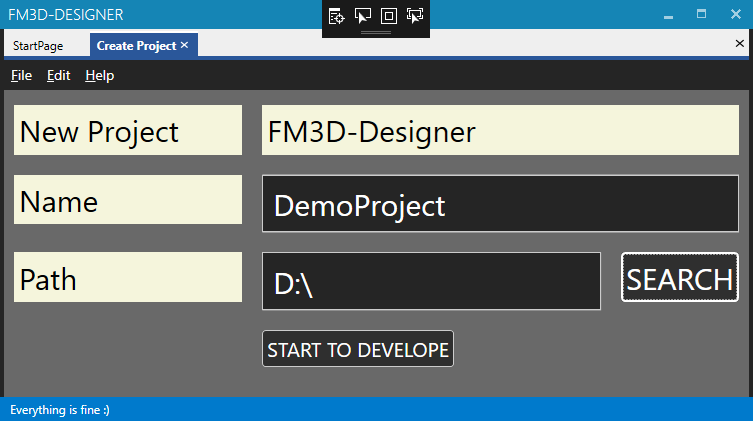
\includegraphics[width=0.5\textwidth]{04verwendung/Designer/00createproject.PNG}.
		\caption{Der Dialog um ein neues Projekt zu erstellen}\label{createprojekt}
	\end{center}
\end{figure}

\subsection{Altes Projekt laden}
\label{projektladen}
Falls Sie nun ein Projekt erstellt haben und es laden wollen, drücken Sie auf die Schaltfläche \textit{Load} rechts neben der Textbox. Es öffnet sich nun ein Explorer-Dialog in dem Sie nun eine \textit{.fmproj} Datei auswählen können. Wenn Sie nun eine Solche ausgewählt haben, drücken Sie auf \textit{Start}. Sie werden nun auf den Haupt-Arbeitsplatz des FM3D-Designers weitergeleitet.
Der Pfad des letzten geladenen Projektes kann durch den ContextMenü Punkt \textit{Last Project} in die Pfadleiste geladen und kann sofort geöffnet werden.

\subsection{Hauptarbeitsplatz}
Wenn sie nun in das Main-Layout (Siehe \cref{mainlayout}) gelangt sind befindet sich rechts ein File-Browser (Siehe \cref{filebrowser}). In diesem werden ihnen nun drei Ordner angezeigt. In diesen können Sie nun beliebig viele Entities und voraussichtlich\todo[inline]{wurk or nut wurk?} Ressourcen in das Projekt laden. Öffnen Sie nun ein Entity um verschiedene Komponente hinzuzufügen.
Auch können Sie Textdateien mit jeder beliebigen Endung zum Projekt hinzufügen.
Die Exportierten Ressourcen müssen Sie manuell in das Cpp Projekt einbinden.
Wenn Sie weitere Ordner in das Projekt einfügen wollen, speichern sie zunächst das Projekt ab und schließen Sie den FM3D-Designer. Gehen Sie dann in ihren Dateiexplorer, öffnen sie den Projektpfad und erstellen Sie an der beliebigen Stelle ein Verzeichnis. Laden Sie das Projekt neu über den Designer und klicken Sie mit der rechten Maustaste auf das Projekt-Item (Siehe \cref{item}). Ein \textit{ContextMenü} öffnet sich nun. Betätigen Sie den Schalter \textit{Include} und die Datei wird zum Projekt hinzugefügt.
\begin{figure}
	\begin{center}
		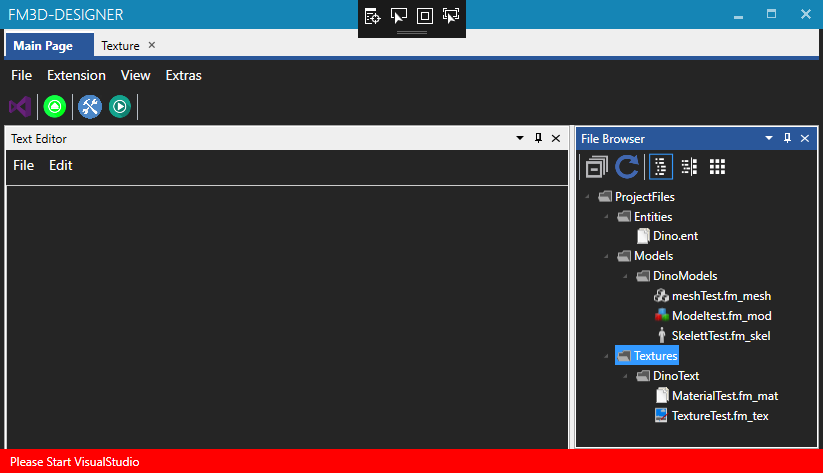
\includegraphics[width=0.5\textwidth]{04verwendung/Designer/01workstation.PNG}
		\caption{Der Haupt-Arbeitsplatz des FM3D-Designers}\label{arbeitsplatz}
	\end{center}
\end{figure}

\subsection{Extension}
Stellen Sie sicher, dass die FM3D-Extension installiert ist und starten sie darauf hin das VisualStudio-Projekt aus dem Designer. Klicken Sie, falls Sie es nicht schon getan haben, hierfür auf das Visual-Studio Icon im Designer. ([1] in \cref{extmen})
Bestätigen Sie die \textit{MessageBox} und warten Sie bis das Projekt geladen wurde.
Wenn es nun geladen wurde, überprüfen Sie nochmal ihre Entities im File-Browser. Falls alle ihren Vorstellungen übereinstimmen, gehen Sie nun auf den zweiten Schalter und betätigen Sie diesen. ([2] in \cref{extmen})
Nun werden die Entity-Preset Klassen in dem VisualStudio-Projekt generiert. Speichern Sie ihr Projekt anschließend.
Wenn sie ihr Spiel fertig Programmiert haben, so können Sie es über das Programm mit den zwei letzten Icons Debugen und Compilen ([3] und [4] in \cref{extmen}), falls Sie noch gerade im Designer beschäftigt sind. Diese Funktion ist optional.
\begin{figure}
	\begin{center}
		
\includegraphics[width=0.2\textwidth]{04verwendung/Designer/02ExtensionMenu.PNG}.
		\caption{Das Extension Menü}\label{extmen}
	\end{center}
\end{figure}
\section{Engine}
\label{verwendung_engine}
Wenn Sie die FM3D-Engine in Kombination mit dem FM3D-Designer verwenden, so wird Ihnen bei der Projekterstellung ein funktionsfähiges VisualStudio C++ Projekt generiert, welches in der VisualStudio-Solution \textit{GameProject.sln} zu finden ist.
Es wird Ihnen geraten, nichts an dem generierten Code zu ändern.
In der Datei \textit{"`presets.h"'} werden die Entity-Presets generiert, welche Sie im Designer erstellen können.
Sie können dem Projekt auch neue Dateien hinzufügen und unabhängig vom generierten Code programmieren. Weitere Dateien, welche ursprünglich nicht zu dem generierten Projekt gehört haben, sollten keinen Einfluss auf die Funktionalität des generierten Codes haben. Das Spiel an sich steht in der \textit{Main.cpp} Datei, welche im Projekt bereits vorhanden ist.

\subsection{Voreinstellungen}
Falls Sie die Engine in Kombination mit dem FM3D-Designer verwenden, so werden die Verzeichnisse automatisch eingebunden. Falls nicht, so müssen Sie Zunächst die Bibliotheken der FM3D-Engine, OpenGL, FreeImage, FreeType und Assimp in das Projekt manuell einbinden. Fügen Sie die Verzeichnisse in die zugehörige Option hinzu. Das ganze sollte so in ihren Einstellungen aussehen:
$$Configuration Properties->C/C++->Additional Include Directories$$\cref{includeinc}
$$Configuration Properties->Linker->Additional Include Directories$$
\cref{liblib}

\begin{figure}
	\begin{center}
		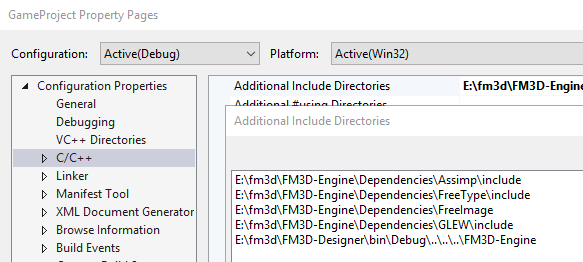
\includegraphics[width=\textwidth]{04verwendung/Engine/include.png}
		\caption{Include Verzeichnisse}\label{includeinc}
	\end{center}
\end{figure}

\begin{figure}
	\begin{center}
		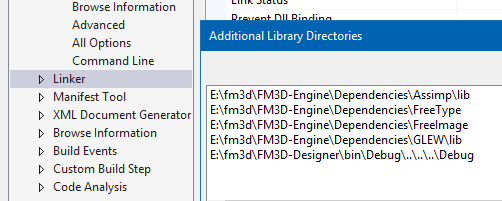
\includegraphics[width=\textwidth]{04verwendung/Engine/lib.png}
		\caption{Lib-Verzeichnisse}\label{liblib}
	\end{center}
\end{figure}

\subsection{Kamera}
Die Kamera ist in dem generierten Projekt bereits vorhanden. Ihnen wird empfohlen die Werte der Position, Rotation, Zoom usw. der Kamera im Bereich der \textit{Game-Logic} zu verändern. Auch dieser Bereich ist eindeutig mit Kommentaren kenntlich gemacht.
In dem erstellten Projekt existiert bereits ein Objekt der Klasse \textit{Camera}. Die \textit{Get}-Methoden geben eine Referenz zu dem jeweiligen Parameter der Kamera. Diese können somit sofort manipuliert werden. Als Beispiel:
\begin{lstlisting}{Cam}
// Create Camera Object
Camera camera(Vector3f(0.3f,0.4f,0.0f));
// Positionattribute Manipulation
camera.GetPosition().x += 0.5f;
camera.GetPosition().y -= 0.1f;
\end{lstlisting}
Für weitere Infos über die Syntax der Kamera wird empfohlen, in der DoxyGen-Dokumentation die Klasse "`Camera"' nachzuschlagen.

\subsection{Entities}
Erstellen Sie zunächst die Entities an der eindeutig kommentierten Stelle \textit{"'Create Entities here"`}. Erstellen Sie beliebig viele Preset-Objekte Ihrer erstellten Entity-Preset-Klassen. Sie können nun bei jedem beliebigen Objekt "`Preset-Einstellungen"' tätigen, in dem Sie dem Entity-Preset-Objekt Standardwerte zuweisen. Gehen wir davon aus, es gäbe ein Entitypreset Namens BaumPreset. Diesem wurde mittels Designer das RenderableComponent hinzugefügt.
\begin{lstlisting}{Entity}
BaumPreset baumpreset1;
\end{lstlisting}
Um nun dem Preset-Objekt ein Standartmodel zuzuweisen, verwendet man die folgende Syntax:

Erstellen wir zunächst ein Referenz-Objekt vom Typ Model.
\begin{lstlisting}{Entity}
Model* baummodel;
\end{lstlisting}
Um nun ein Model zu laden, wird die Klasse \textit{ExternFileManager} wie folgt verwendet:
\begin{lstlisting}{Entity}
ExternFileManager::
ReadModelFile("res/baum.dae", rendersystem, &baummodel, false, true);
\end{lstlisting}
Dies sagt nun Folgendes aus:
wir übergeben den Dateipfad "`res/baum.dae"' und ein Objekt des Render-Systems, in dem dann das Model gerendert werden soll. Daraufhin wird eine Adresse zu dem Objekt der Klasse \textit{Model} übergeben, in der das Model gespeichert wird. Der darauffolgende boolesche Wert gibt an, ob Instancing verwendet werden soll und der folgende, ob das Modell animierbar sein soll. Sie können nun dem Objekt Baum dieses Standartmodel zuweisen. Dies geschieht wie folgt:
\begin{lstlisting}{Entity}
baumpreset1.SetModel(&baummodel);
\end{lstlisting}
Initialisieren Sie nun einen Entity-Pointer (Klasse: \textit{EntityPtr}) und erstellen Sie das Entity in der bereits initialisierten \textit{EntityCollection} namens \textit{scene}. Als Beispiel:
\begin{lstlisting}{Entity}
EntityCollection scene;
EntityPtr baum = scene.CreateEntity();
\end{lstlisting}
Ein Objekt der Klasse \textbf{EntityCollection} beinhaltet alle Entities, die in dem Spiel verwendet werden. Jedoch können auch mehrere EntityCollection erstellt und verwendet werden.
Um die Presets auf einen Entity-Pointer und somit auf ein Entity in einer EntityCollection anzuwenden, wird die folgende Syntax verwendet:
\begin{lstlisting}{Entity}
baumpreset1.SetComponents(baum);
\end{lstlisting}
Nun wird dem EntityPointer alle Komponenten, mit den zuvor zugewiesenen Standartwerten, zugewiesen.

Wenn ein Entity das Komponent \textit{RenderableComponent} besitzt, so kann es in dem eindeutig kommentierten Abschnitt "`Submit objects here to renderer"' dem Renderer übergeben werden. Das heißt nun, dass das Model des Entities gerendert werden kann.
\begin{lstlisting}{Entity}
/// ##########################
  //
  //  Submit objects here to renderer!
  //
  renderer3D-Submit(baum.get());
/// ##########################
\end{lstlisting}
Bevor Sie den Entities die Modelle zuweisen, vergessen Sie nicht die Modelle in die Projektmappe von VisualStudio zu laden.

\subsection{Inputsystem}
\label{inputsystemver}
Hierfür wird die Klasse \textit{Input} verwendet. Möchte man nun Tasten abfragen, so muss man zunächst über das Fenster auf das Objekt der Klasse Input zugreifen. 
Nun kann eine Methode aus dieser Klasse verwendet werden.
Möchten Sie nun abfragen, ob z.B. die Taste F5 auf der Tastatur gedrückt wurde, so schreiben Sie dies so in den Code:
\begin{lstlisting}{Input}
win->GetInput().CheckKey(KEY_F5);
\end{lstlisting}
Möchten Sie nun überprüfen, ob die Linke Maustaste gedrückt wurde, so tun Sie dies folgendermaßen:
\begin{lstlisting}{Input}
win->GetInput().CheckMouse(MOUSE_LEFT);
\end{lstlisting}

Möchte man nun die Position des letzten Klicks der linken Maustaste ermitteln, benutzt man diese Methode:
\begin{lstlisting}{Input}
win->GetInput().GetLastposClick(MOUSE_LEFT);
\end{lstlisting}
Diese gibt einen zweidimensionalen Vektor vom Typ Float zurück, welcher die Position vom letzten Klick der Maus mit einer bestimmten Maustaste beschreibt. 
Die folgende Methode gibt Daten in Form eines zweidimensionalen Vektors mit der aktuellen Position der Maus zurück:
\begin{lstlisting}{Input}
win->GetInput().GetLastposInst();
\end{lstlisting}

Alle Tasten der Tastatur und Maus können über Makros angesprochen werden. Auch können Sie die ASCII-Codes der einzelnen Tasten verwenden. Die Makros, welche die Tasten der Tastatur beschreiben, starten mit \textit{"`KEY\_"'}. Die Makros, die für die Maus verwendet werden, starten mit \textit{"`MAUS\_"'}.
(Für weitere Informationen: Siehe DoxyGen Dokumentation)